\begin{center}\begin{tabular}{lrrr}\toprule
Sample & $N_g$ & $a_0/(10^{-10}\,\mathrm{m\,s^{-2}})$ & $\chi^2/(N-k)$\\\midrule
all & 153 & 1.250 & 4.842\\
gas dominated & 66 & 1.000 & 2.617\\
star bulgeless & 56 & 0.900 & 4.375\\
star bulge & 31 & 1.900 & 6.574\\
star bulge deep & 25 & 1.600 & 3.903\\
star bulgeless deep & 50 & 0.850 & 1.815\\
\bottomrule\end{tabular}\end{center}
These are grid minima from fresh penalized profiles, not Bayesian posterior estimates.
The descriptive reduced chi-square values expose substantial fit inadequacy.
The fixed stellar RAR reference gives $a_0=1.2216\times10^{-10}$ m s$^{-2}$.
Planck base LCDM: externally propagated $a_{0,H}=(1.04220\pm 0.00773)\times10^{-10}$ m s$^{-2}$.
SH0ES Cepheid-SN: externally propagated $a_{0,H}=(1.12941\pm 0.01608)\times10^{-10}$ m s$^{-2}$.
Removing UGC06787 shifts the deep-bulge grid optimum from $1.60$ to $0.90$ in units of $10^{-10}$ m s$^{-2}$. An independent full-grid refit of 24 galaxies and 287 points confirms this influence diagnostic. This does not justify excluding the galaxy or claiming nonuniversality.
The maximum forward/reverse total-objective difference is 4.74029e-09.
Full numerical profiles, conditional crossings, influence ranges and sensitivity variants are in \texttt{docs/SPARC\_FRESH\_RESULTS.md} and the JSON artifact.
No $\Delta\mathrm{BIC}$ or calibrated discovery significance is asserted. External $H_0$ uncertainty is not integrated in these profiles.
\begin{figure}[ht]\centering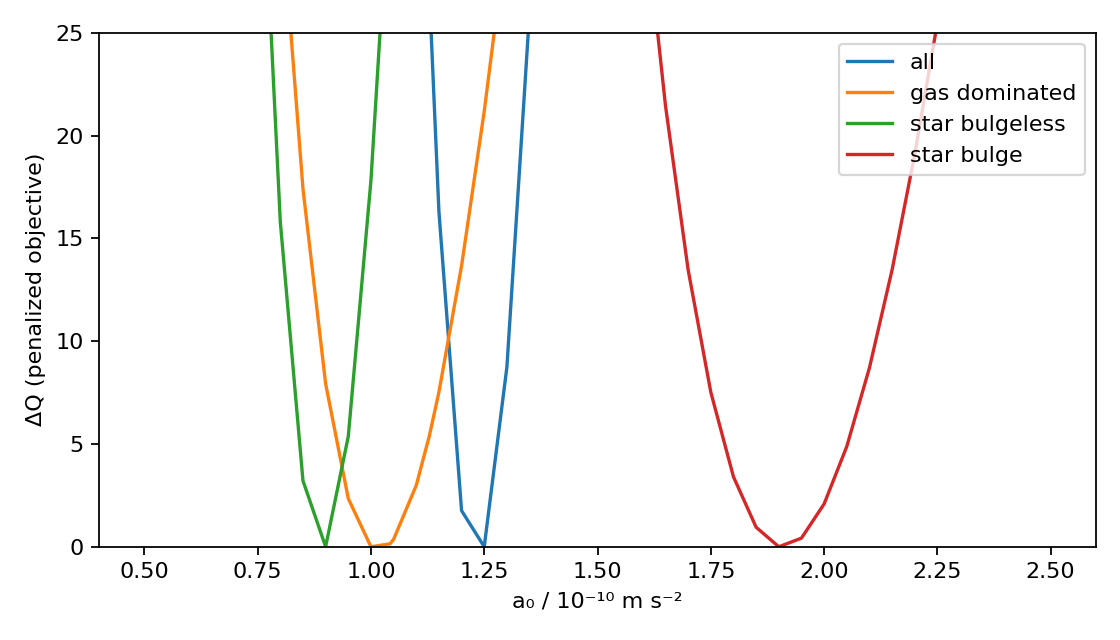
\includegraphics[width=.85\linewidth]{figures/sparc_fresh_profiles.png}
\caption{Fresh penalized objective profiles. The plotted differences are not discovery significances.}\end{figure}
